\documentclass[10pt, a4paper]{article}
% The next line loads some packages you will need

\usepackage{graphicx, amsmath, amssymb, fancyhdr, setspace,titlesec,enumitem,indentfirst,hyperref}
\usepackage[labelfont=bf]{caption}
\hypersetup{
    colorlinks=true,
    linkcolor=blue,
    filecolor=blue,      
    urlcolor=cyan,
    pdftitle={Overleaf Example},
    pdfpagemode=FullScreen,
    }

% Page formatting
\addtolength{\textwidth}{5mm}
\addtolength{\textheight}{12mm}
\addtolength{\topmargin}{-10mm}
\pretolerance = 10000000
\setlength{\parindent}{23pt}
% \setlength{\parskip}{\baselineskip}
\onehalfspacing   

% Header / footer
\pagestyle{fancy}
\lhead{Himanshu Madan, 201501359}
\chead{}
\rhead{\em MATH 5747M, assignment 2}
\lfoot{}
\cfoot{\thepage}
\rfoot{}
\setlength{\headheight}{20pt}
\renewcommand{\headrulewidth}{0.4pt}
\renewcommand{\footrulewidth}{0pt}

% \titlespacing\section{0pt}{10pt plus 4pt minus 2pt}{0pt plus 0pt minus 0pt}

\begin{document}
\begin{center}
\textbf{\Large Decision Science Using MCDA} \\
Based on module LUBS 5308M Business Analytics and Decision Science \\
Lectured by Dr. Richard Hodgett \\
\end{center}

\section*{Introduction}
The objective of this report is to explain two different but prominent \textbf{Multi Criteria Decision Analysis} techniques:
\begin{itemize}[noitemsep]
    \item \textbf{Analytic Hierarchy Process }(AHP)
    \item \textbf{Technique for Order Preference by Similarity to Ideal Solutions }(TOPSIS)
\end{itemize}
MCDA techniques allow us to choose the most suitable alternative amongst all the options available using the information available.\\
In MCDA, we have :
\begin{enumerate}[noitemsep]
    \item A goal to be achieved. Ex: choose a car to buy.
    \item Multiple alternatives available. Ex: Ford Fiesta, Audi A8, BMW 530d.
    \item Several criteria influencing our decision making. Ex: cost, engine power etc.
\end{enumerate}
\begin{figure}[h]
	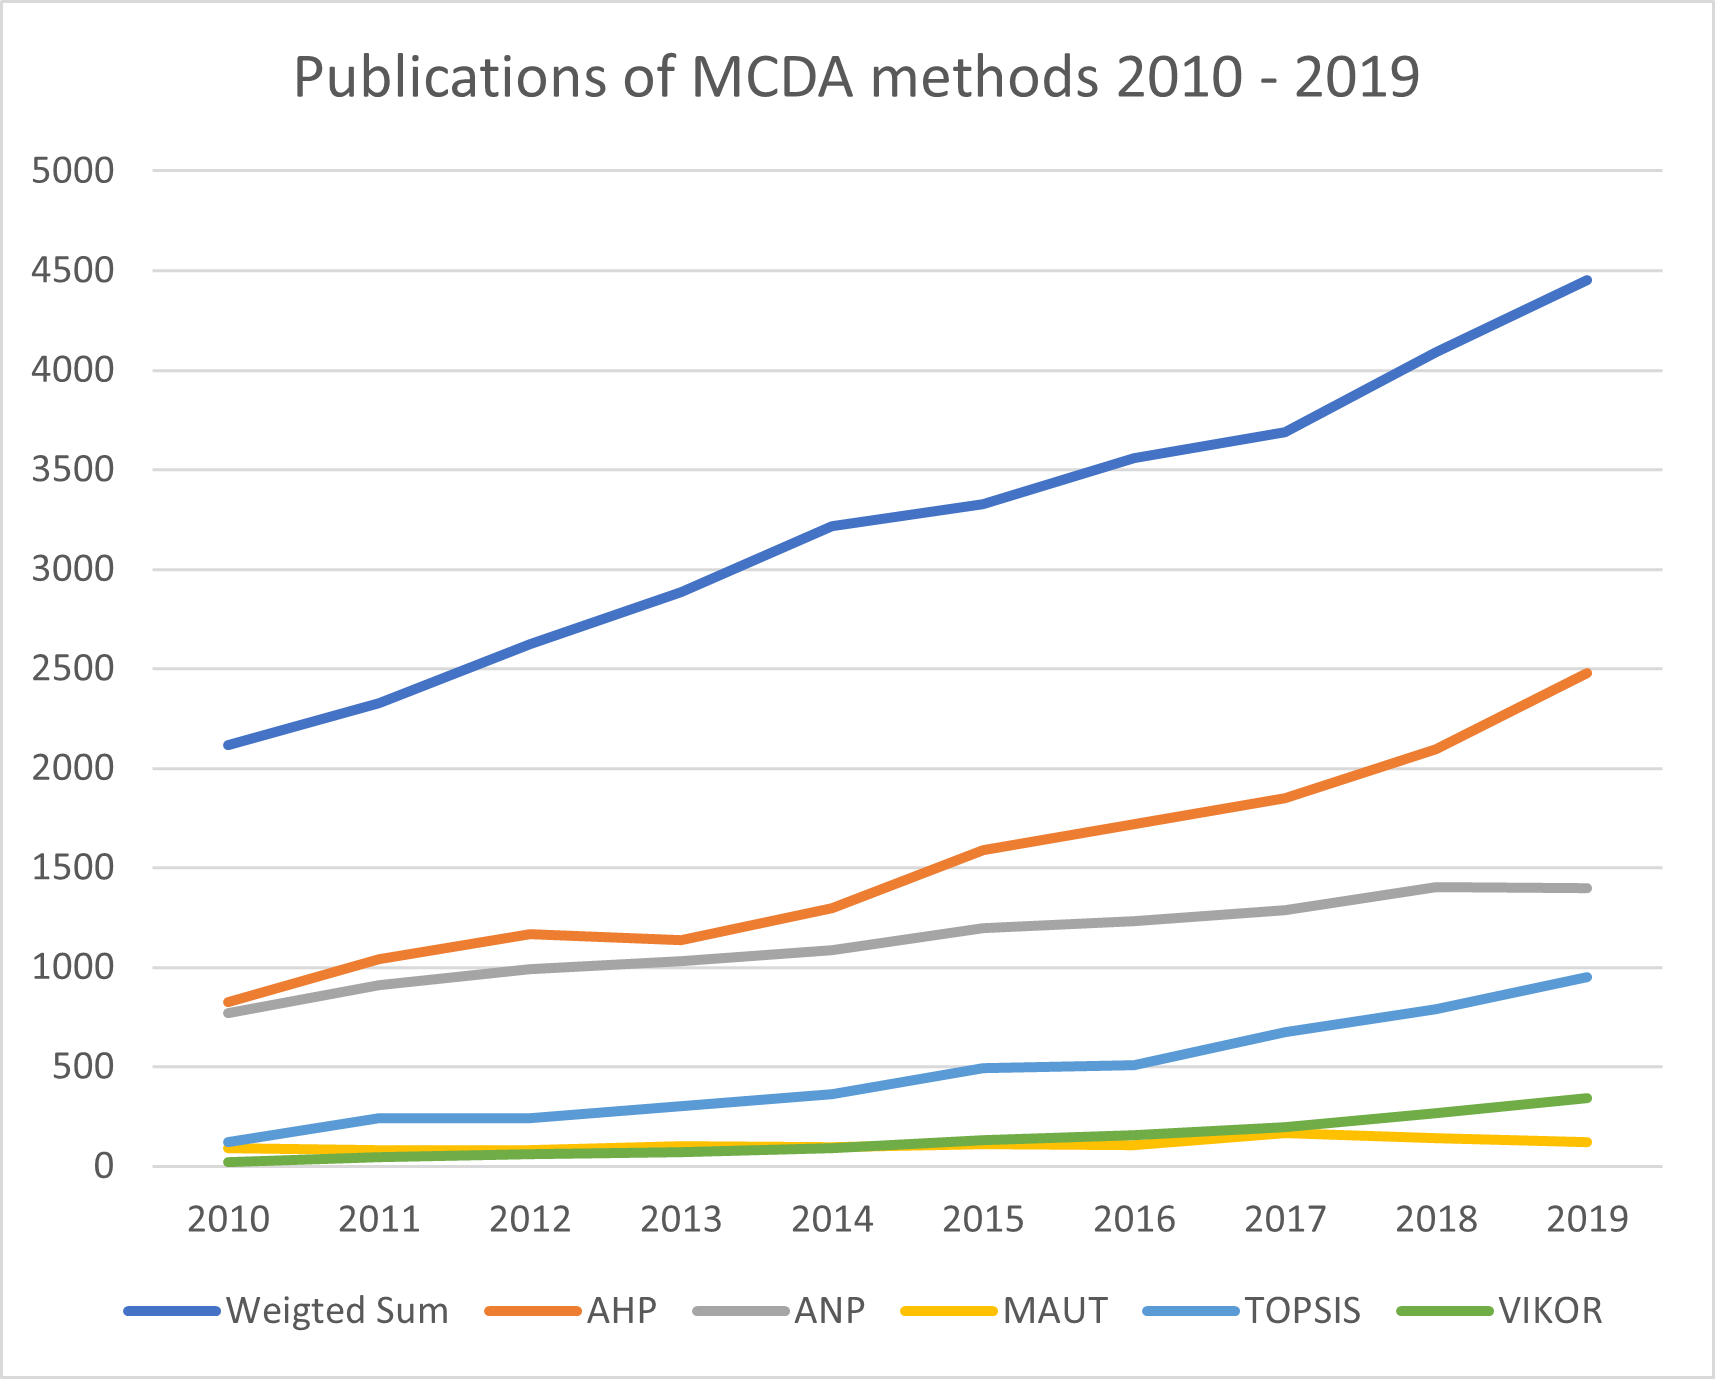
\includegraphics[width=9.5cm]{LUBS5308M Week03 Img001 - MCDA Methods}
	\centering
	\caption{Research outputs showing growing popularity of different MCDA techniques. (Source: Module Learning Material, Week 3)}
    \end{figure}

As the name implies, MCDA allows you to consider multiple conflicting criteria and decide on the best option using different types of information. 
Decisions are incredibly important in industry, especially decisions related to product development.\\
In the following sections, we will understand AHP and TOPSIS one by one with examples.
\section{Analytic Hierarchy Process}
 AHP is a pairwise comparison method, which is an approach to MCDA, in which we compare each alternative/criterion head-to-head with all the other alternatives/criteria and it is up to the decision maker to choose the best comparison.\\
 It was given by \underline \href{https://en.wikipedia.org/wiki/Thomas_L._Saaty}{Prof. Thomas Saaty} in 1970. 
There are two approaches to elicit scores from the reciprocal matrix:
\begin{enumerate}[noitemsep]
    \item Eigenvector method
    \item Geometric mean method
\end{enumerate}
\end{document}
